\documentclass[titlepage]{article}
\newcommand{\var}{\textrm{Var}}
\newcommand{\E}{\textrm{E}}
\newcommand{\Normal}{\mathcal{N}}
\newcommand{\Ito}{It\^{o}~}

\usepackage{amsmath, amsthm, amssymb}
\usepackage[pdftex]{graphicx}
\usepackage{epstopdf}

%IEEE compliance:
\DeclareGraphicsRule{.eps}{pdf}{.pdf}{`epstopdf --gsopt=-dPDFSETTINGS=/prepress #1}

\author{Yuriy Sverchkov}
\title{Modeling Flagellar Growth as a Stochastic Process}

\newtheorem*{clthm}{Central Limit Theorem for Renewal Processes}
\newtheorem*{itoform}{The \Ito Formula}

\begin{document}

%\maketitle

\begin{titlepage}
\begin{center}

\vspace*{2.5in}
{\Large Modeling Flagellar Growth as a Stochastic Process}

\vspace{0.5in}
{\large Yuriy Sverchkov}

\vfill
{\Large Senior Thesis\\ }

\vspace{0.25in}
{\large Advisor: Dr. Muruhan Rathinam

\vspace{0.25in}
Mathematics Department\\ University of Maryland, Baltimore County}

\vspace{0.5in}
\today

\end{center}
\end{titlepage}

\section{Introduction}

Some of the important questions in cellular biology have to do with how the sizes of different parts of the cell, the organelles, are regulated.
Here we concentrate on modeling the growth of the Eukaryotic flagellum, an organelle that protrudes from the cell and is usually used for propulsion.
The choice of studying a flagellum has the advantage of restricting the problem to growth in only one dimension.
~\cite{bressloff}

\begin{figure}[!ht]
\centering
\parbox[t][2.3in][t]{4in}{
\hspace{1in}IFT Particles\\
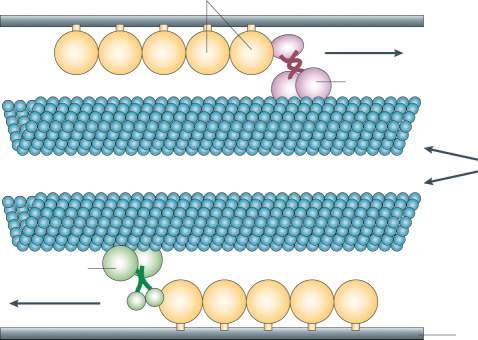
\includegraphics[width=3in]{IFT_diagram.png}
\raisebox{1.75in}[1pt][1pt]{\hspace{2.2in}Kinesin-II}\\
\raisebox{1.39in}[1pt][1pt]{\hspace{3.04in}Microtubules}\\
\raisebox{1.5in}[1pt][1pt]{($-$)\hspace{2.2in}($+$)}\\
\raisebox{1.05in}[1pt][1pt]{\hspace{-0.15in}Dynein-1b}\\
\raisebox{0.83in}[1pt][1pt]{\hspace{2.95in}Flagellar membrane}
}
\caption{The interflagellar transport machinery.~\cite{rosenbaum2}
During intraflagellar transport,
linear arrays of IFT particles (yellow) are anterograde,
towards the ($+$) ends of the flagellar microtubules (blue)
by kinesin-II (pink), and retrograde (towards the ($-$) ends)
by cytoplasmic dynein 1b (green).
The IFT particles carry precursors that are necessary for the assembly of
the flagellar axoneme.}
\end{figure}

Eukaryotic flagella grow using the mechanism of intraflagellar transport. This process describes the movement of particles (transporters) carrying building blocks (precursor proteins) along the microtubule and depositing them at the flagellum tip.
The transporters use different motors for anterograde (towards tip) movement and retrograde (towards cell body) movement.
~\cite{rosenbaum}

In order to express the length of the flagellum mathematically we define the relevant variables as follows:
$L$ represents the flagellar length, $a$ represents the effective size of a precursor protein transported by a transporter, $v_+$ represents a transporter's anterograde speed, $v_-$ represents a transporter's retrograde speed, and $M$ represents the number of transporters in the flagellum.
We also suppose that a flagellum degrades at a constant speed of $V$.
Using these parameters it is possible to arrive at an ordinary differential equation (ODE) for the flagellum length, at the microscopic level, however, a stochastic model may be more representative of the behavior of the motors and transporters.
Our goal is to represent flagellar growth as a stochastic process, and compare and contrast the stochastic model with the deterministic model.
We are also interested in analyzing the behavior that cannot be predicted by the deterministic model, such as the variation of the flagellum length.
The deterministic ODE for the flagellum length is:

\begin{equation*}
\frac{dL}{dt} = \frac{a \bar{v} M}{2L} - V
\end{equation*} 

Where $\bar{v}$ is the harmonic mean of $v_+$ and $v_-$.
The assembly rate, which is the positive right-hand-side term, is arrived at by noting that a transporter adds a segment of length $a$ to the flagellum every time it completes one round trip, to the tip of the flagellum and back.
The time it takes to complete this trip is the time taken to reach the tip from the base, $L/v_+$, added to the time it takes to reach the base from the tip, $L/v_-$, adding up to $2L/\bar{v}$.
The disassembly rate is given by $V$ and is length-independent.

The values we use for the parameters above in our simulations are taken from the paper by Paul C. Bressloff, \emph{Stochastic model of intraflagellar transport }~\cite{bressloff}: $v_+$, $v_-$, and $V$ are taken to be $2.0 \mu$m$/$s, $3.5 \mu$m$/$s, $0.01 \mu$m$/$s respectively, $M$ is taken to be 10, and $a$ is taken to be $10$nm.


\section{Discrete Stochastic Model}
\label{sec:OriginalModel}

Following an approach similar to \cite{bressloff},
we model the process as a discrete-state continuous-time Markov process as follows:
We view the flagellum as having $N = L / a$ segments.
Each transporter has a position between $0$ (the flagellum base) and $N$ (the flagellum tip).
We also keep track of the direction of a transporter.
If a transporter $i$ ($i=1,...,n$) is moving anterograde, we consider the time it takes it to move from position $x$ to its next position $x+1$ to be an exponential random variable $T_{i,x+}$ with rate $\lambda_+ = v_+ / a$.
Similarly,  retrograde  movement from position $x$ to position $x-1$ is represented by discrete jumps a random exponential time period $T_{i,x-}$ apart (with a rate of $\lambda_- = v_- / a$).
Disassembly is similarly represented by a discrete shortening of the flagellum length at random exponentially distributed time intervals $S$ with the corresponding rate of $\mu = V / a$.
The direction of movement of a transporter changes only at the tip and at the base as follows:
When a transporter at the tip (position $N$) is moving anterograde jumps to its next position, $N$ is incremented, the transporter's new position is the new value of $N$, and its direction of movement becomes retrograde.
When a transporter at position $1$ is moving retrograde jumps to its next position, its new position becomes $0$ and its direction becomes anterograde.

Note that the resulting state-space for this Markov process has $M+1$ dimensions.


\subsection{Monte Carlo Simulation}

The most intuitive way to simulate a Markov Process is through the means of a Monte Carlo method, by generating values for the random variables $T_{i,x-}$, $T_{i,x+}$ and $S$ with a pseudorandom number generator (PRNG) and using those values to simulate the positions of the transporters and the flagellum length at any given moment in time.

We have encountered some challenges regarding the implementation of the simulation due to the number of steps the simulation must take to simulate a reasonably long time period.
Initially, MATLAB was used for the simulation. However, the MATLAB simulation took an unreasonably long period of time to run, and the simulation had to be re-written in C.
The C code ran considerably faster.
In writing the simulation code it was also important to make sure that the simulation does not exceed the PRNG's period.
In our simulation, we used the SIMD-oriented Fast Mersenne Twister algorithm~\cite{matsumoto} with a period of $2^{216091}-1$ iterations.
The number of random numbers generated per simulation run is as follows:
A step (a transporter moves or the flagellum shortens) occurs between $10 \times 350+1$ and $10 \times 200+1$ times per simulation second.
Two random numbers are generated per step: one to select the event that happens, and one to determine the waiting time until the next event.
We run simulations with time limits of $15000$ and $50000$ simulation seconds, resulting in about $10^7$ to $10^8$ random numbers generated per each trajectory.
Adding that we would like to get final distributions by running thousands of trajectories, and then compare several such sets of runs, adds three or more orders of magnitude to the number of random numbers to be generated.


\subsection{Trajectories}
At first glance, the stochastic IFT model seems to be in agreement with the ODE model. Figure~\ref{fig:originalTrajs} shows some sample trajectories created by the simulation with their ODE solution counterparts.

\begin{figure}[!h]
\centering
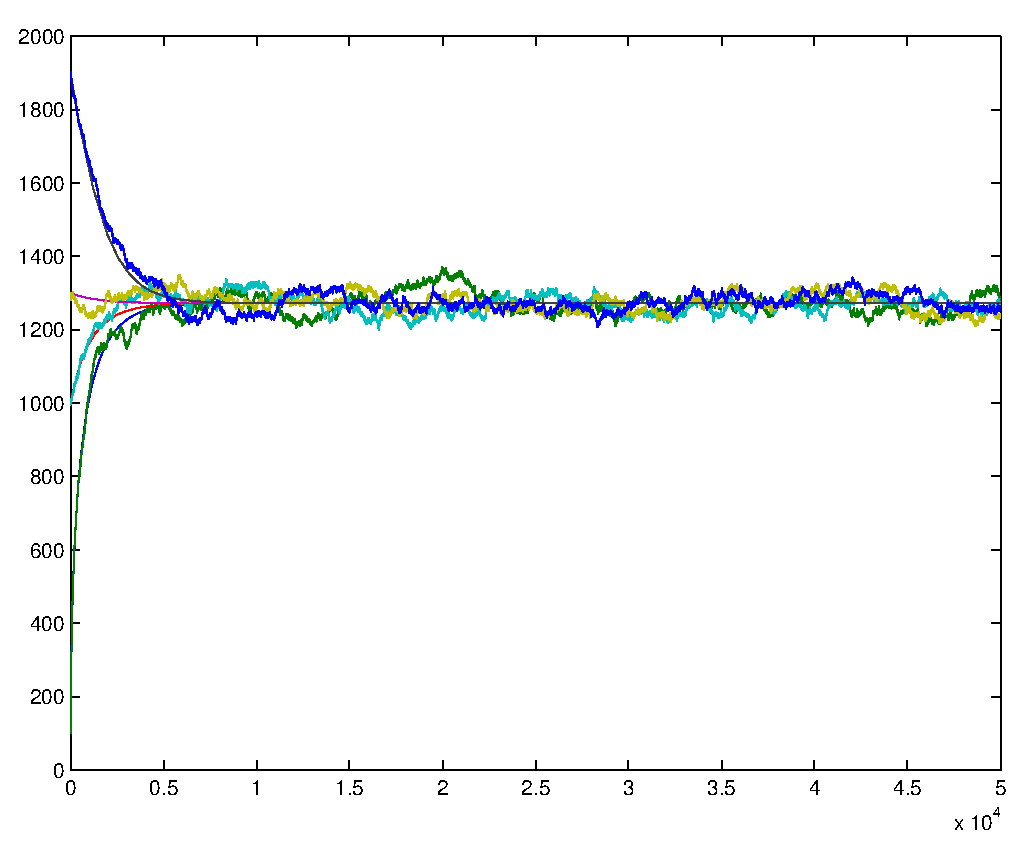
\includegraphics[width=\textwidth]{OriginalModelTrajs}
\caption{
Four representative trajectories generated by the stochastic IFT simulation and corresponding solutions to the ODE.
The four different trajectories start from four different initial lengths: 100, 1000, 1300, and 1900, running to a time limit of 50000.
}
\label{fig:originalTrajs}
\end{figure}

\subsection{Distribution at a Given Time}
%Table~\ref{tab:original} shows
Figure~\ref{fig:orig_ic8_15Ks} shows data from running the simulation of 5000 independent trajectories starting with the same initial conditions and taking the length at a particular predetermined time (15000 simulation seconds in this case).
%See Table~\ref{tab:ic} for a list of initial conditions. Sets of initial conditions were generated so that the IFTs are distributed uniformly.

%\begin{table}[t]
%\centering
%\begin{tabular}{crr}
%Name & Initial Length & Number of IFTs \\ \hline
%ic2 & 100 & 10 \\
%ic5 & 1300 & 10 \\
%ic8 & 1300 & 10
%\end{tabular}
%\caption{List of names for the different sets of initial conditions used for %simulations.}
%\label{tab:ic}
%\end{table}

%\begin{table}[!htbp]
%\centering
%\begin{tabular}{c*6{r}}%{cc*6{r}}
% Fig. &
% I.C. &
% \parbox{50pt}{Time Limit (seconds)} &
% \parbox{40pt}{Number of Runs} &
% Mean &
% \parbox{50pt}{Standard deviation} &
% Skewness &
% Kurtosis
%\\ \hline
% \ref{fig:orig_ic5_50Ks} &
%  ic5 & 50000 & 1200 & 1272.1 & 25.3665 & 0.0294 & 3.1540 \\
% \ref{fig:orig_ic8_15Ks} &
%  ic8 & 15000 & 5000 & 1273.3 & 25.2790 & 0.0045 & 2.8647 \\
% \ref{fig:orig_ic8_50Ks_1} &
%  ic8 & 50000 & 1800 & 1272.3 & 24.7195 & 0.1595 & 3.0236 \\
% \ref{fig:orig_ic8_50Ks_2} &
%  ic8 & 50000 & 2400 & 1273.1 & 25.1025 & 0.0554 & 2.9257 \\
% \ref{fig:orig_ic2_50Ks} &
%  ic2 & 50000 & 3500 & 1271.9 & 25.1562 & 0.0442 & 2.9342 \\
% \ref{fig:orig_ic2_15Ks} &
%  ic2 & 15000 & 5000 & 1273.0 & 25.3101 & -0.0020 & 2.9549

%\end{tabular}
%\caption{Data from ensemble runs of the IFT simulation.}
%\label{tab:original}
%\end{table}

%\begin{figure}[!htbp]
%\centering
%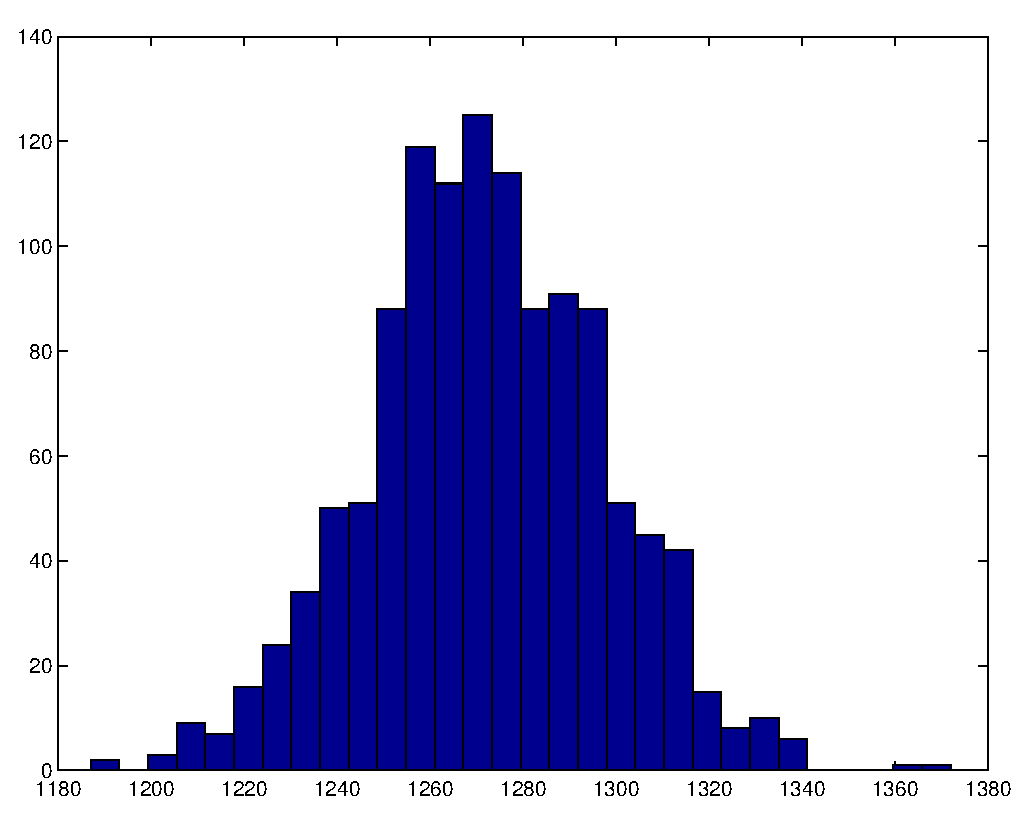
\includegraphics[width=\textwidth]{ic5_50Ks.eps}
%\caption{Distribution of final lengths given by the original simulation. See Table~\ref{tab:original} for details. 30 bin histogram for a sample of 1200.}
%\label{fig:orig_ic5_50Ks}
%\end{figure}

\begin{figure}%[!htbp]
\centering
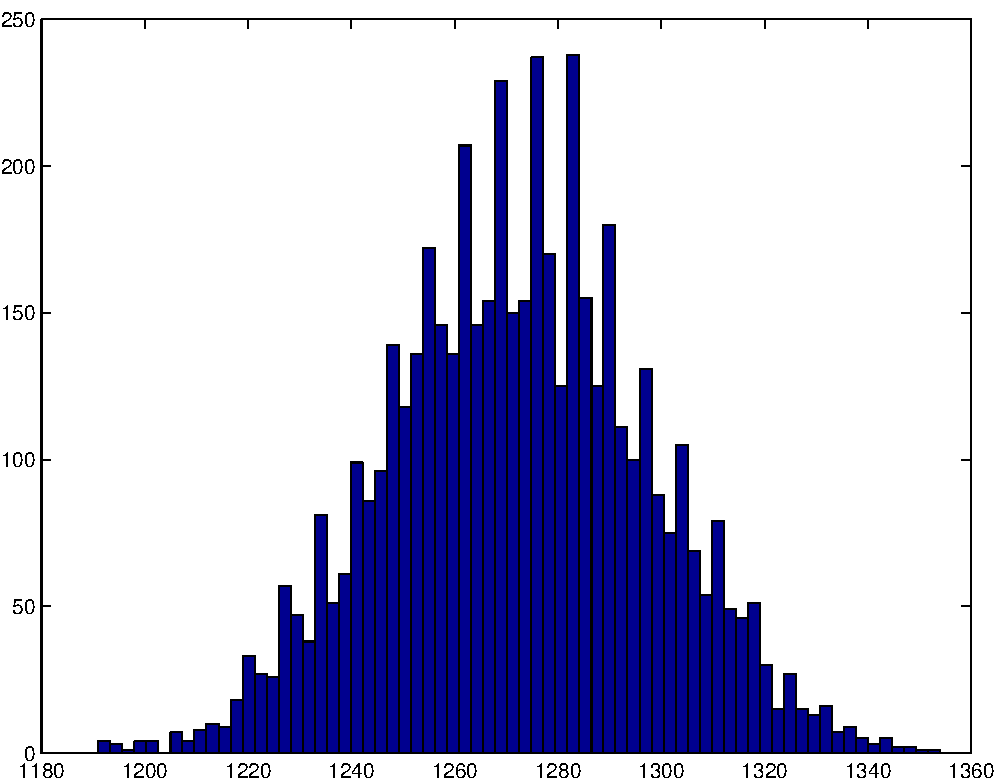
\includegraphics[height=3in]{ic8_15Ks}
\caption{Distribution of final lengths given by the original simulation. The simulation was initialized at an initial length $N(0) = 1300$. 70 bin histogram for a sample of 5000.}
\label{fig:orig_ic8_15Ks}
\end{figure}

%\begin{figure}[!htbp]
%\centering
%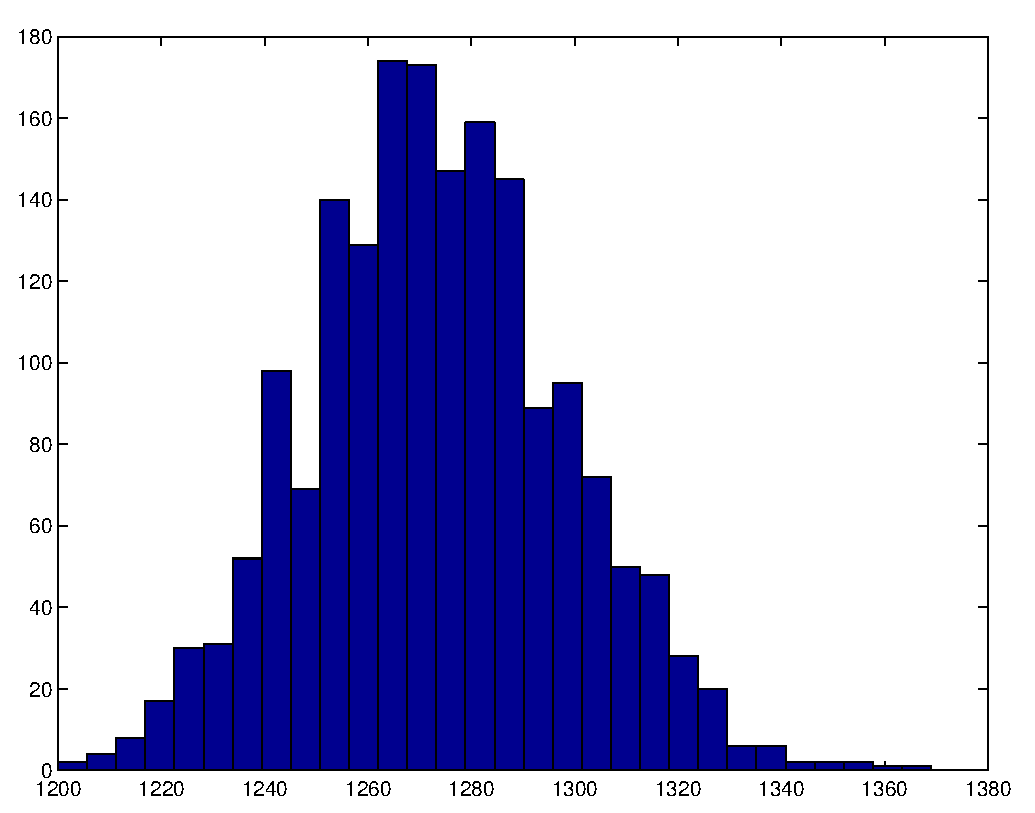
\includegraphics[width=\textwidth]{ic8_50Ks.eps}
%\caption{Distribution of final lengths given by the original simulation. See Table~\ref{tab:original} for details. 30 bin histogram for a sample of 1800.}
%\label{fig:orig_ic8_50Ks_1}
%\end{figure}

%\begin{figure}[!htbp]
%\centering
%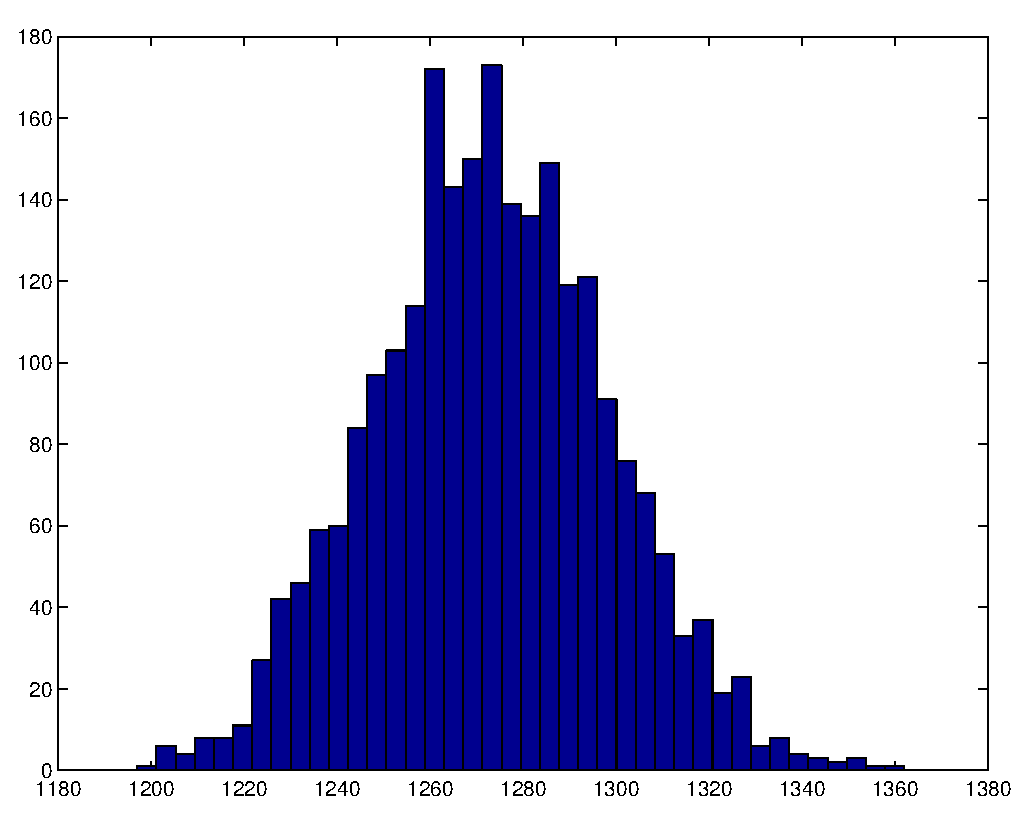
\includegraphics[width=\textwidth]{ic8_50Ks_2.eps}
%\caption{Distribution of final lengths given by the original simulation. See Table~\ref{tab:original} for details. 40 bin histogram for a sample of 2400.}
%\label{fig:orig_ic8_50Ks_2}
%\end{figure}

%\begin{figure}[!htbp]
%\centering
%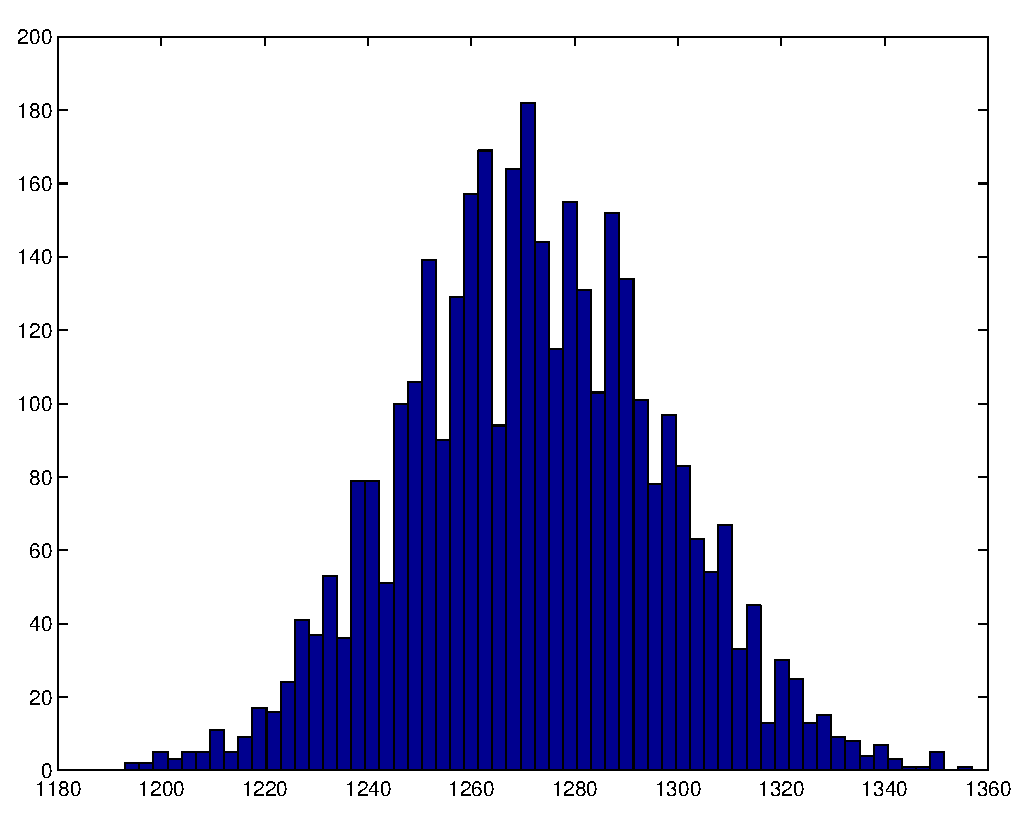
\includegraphics[width=\textwidth]{ic2_50Ks.eps}
%\caption{Distribution of final lengths given by the original simulation. See Table~\ref{tab:original} for details. 50 bin histogram for a sample of 3500.}
%\label{fig:orig_ic2_50Ks}
%\end{figure}

%\begin{figure}%[!htbp]
%\centering
%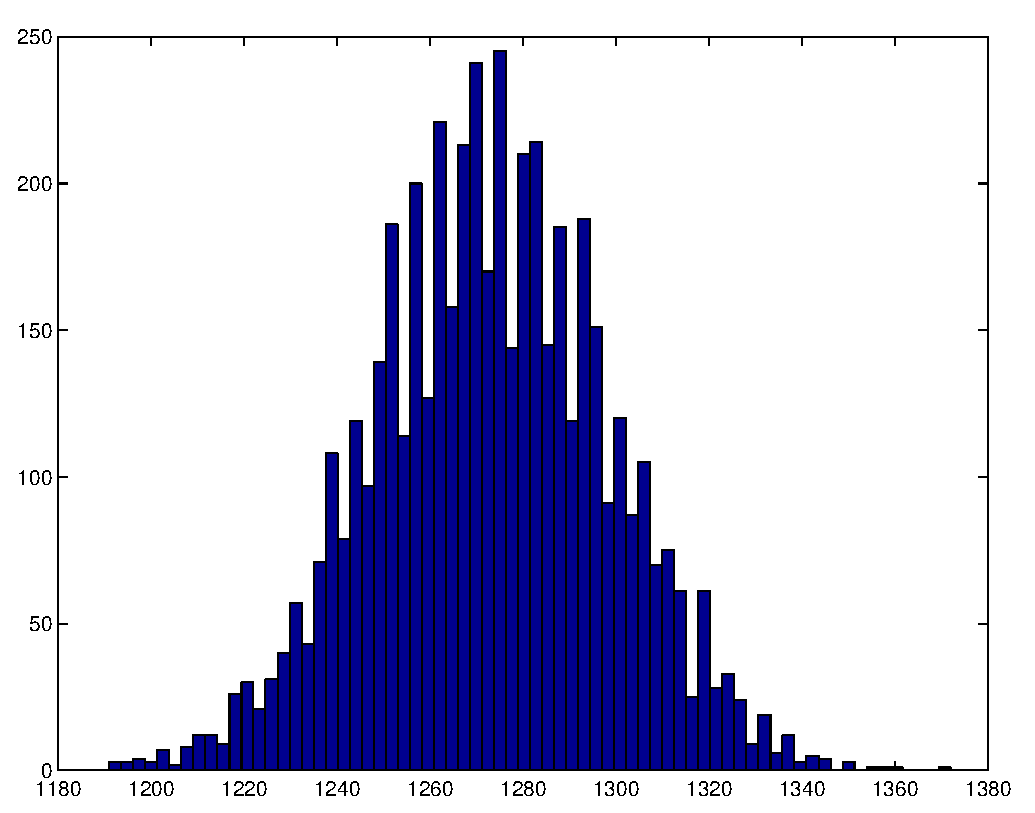
\includegraphics[height=3in]{ic2_15Ks.eps}
%\caption{Distribution of final lengths given by the original simulation. The simulation was initialized at an initial length $N(0) = 1300$. 70 bin histogram for a sample of 5000.}
%\label{fig:orig_ic2_15Ks}
%\end{figure}

\subsection{Comparing Different Distributions}
We generated multiple sets of data with the simulation starting at various initial lengths $N(0)$.
We also compared simulations with time limits of both 50000 and 15000 seconds.

Using the Kolmogorov-Smirnov test (the MATLAB \texttt{kstest2} command) to compare the distributions given by the simulation we can conclude several things:

Since the test cannot reject the hypothesis that the samples come from the same distribution when comparing two samples from different initial lengths and identical time limit shows that starting at different initial conditions leads to the same stationary probabilities as suggested by the trajectory plots.
%(Comparing the distribution in Figure~\ref{fig:orig_ic2_50Ks} to the distribution in Figure~\ref{fig:orig_ic5_50Ks} or Figure~\ref{fig:orig_ic8_50Ks_1} or Figure~\ref{fig:orig_ic8_50Ks_2})

The test also cannot reject the hypothesis when comparing two samples with different time limits (50000s vs. 15000s), leading to believe that the stationary probabilities are reached before 15000s, as suggested by the trajectory plots.
%(Comparing the distribution in Figure~\ref{fig:orig_ic8_15Ks} to the distribution in Figure~\ref{fig:orig_ic5_50Ks} or Figure~\ref{fig:orig_ic8_50Ks_1} or Figure~\ref{fig:orig_ic8_50Ks_2})

%In fact, the test cannot reject the hypothesis when comparing any pair of distributions from Table~\ref{tab:original}.

\subsection{The Crowding Model}
The crowding model is a modified version of the original model with the major difference being that transporters are not allowed to occupy the same position at the same time. This is accomplished by adding a check every time a transporter is selected to move---if there is another transporter in the position in front of it, the transporter does not move. When the flagellum length decreases, transporters are bumped back (that is, if there is an transporter at the very end and another directly behind it, both are moved back).

\subsubsection{Trajectories}
Figure~\ref{fig:crowdTrajs} shows some sample trajectories created by the simulation with their ODE solution counterparts. Visually, the crowding model also apparently agrees with the ODE model.

\begin{figure}%[!htbp]
\centering
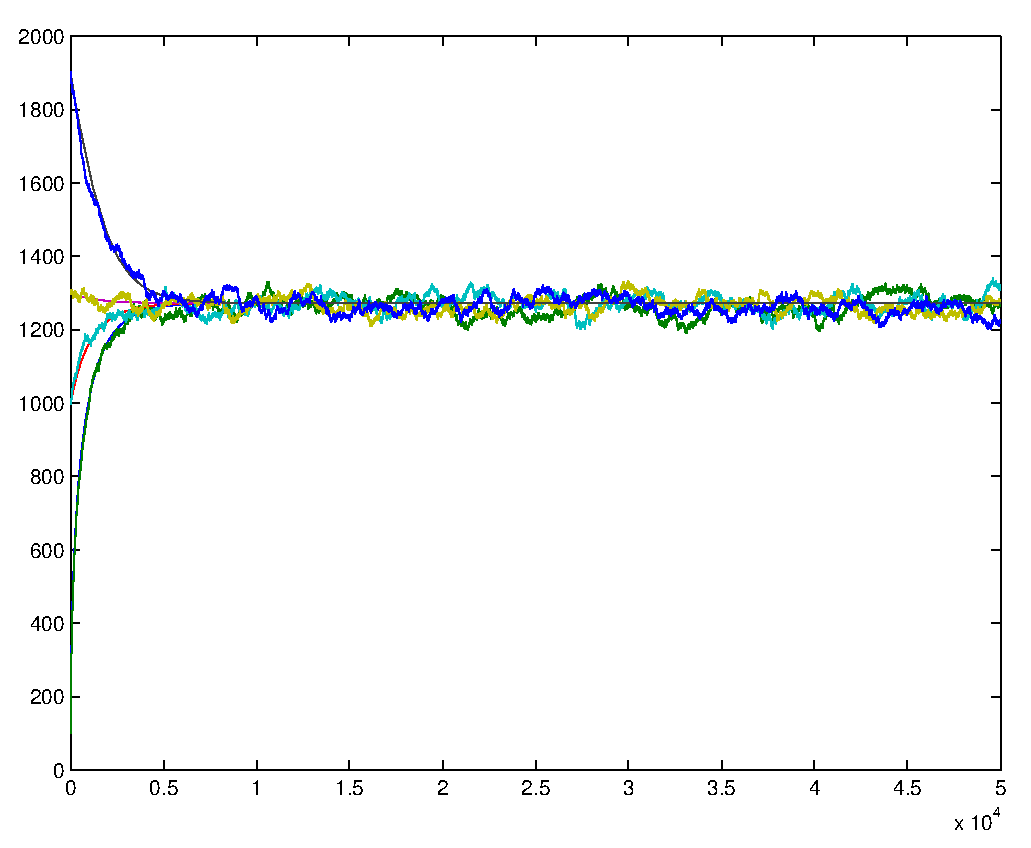
\includegraphics[width=\textwidth]{CrowdingModelTrajs}
\caption{
Four representative trajectories generated by the stochastic IFT simulation with crowding and corresponding solutions to the ODE.
The four different trajectories start from four different initial lengths: 100, 1000, 1300, and 1900, running to a time limit of 50000.
}
\label{fig:crowdTrajs}
\end{figure}

\subsubsection{Distribution at a Given Time}
Figure~\ref{fig:crowd_ic8_15Ks} shows data from running the simulation repeatedly starting with the same initial conditions and taking the length at a particular predetermined time (15000s).
The dataset shown in Figure~\ref{fig:crowd_ic8_15Ks} had a mean of 1268.6 and a standard deviation of 25.4275,
with 95\% confidence intervals of [1268.0, 1269.2] and [25.0211, 25.8474] for the mean and standard deviation respectively.
When compared to the non-crowding model simulation results (see Table~\ref{tab:ci} on page~\pageref{tab:ci}) it can be seen that the crowding model yields a lower mean, but a similar standard deviation.

%\begin{table}[!htbp]
%\centering
%\begin{tabular}{c*6{r}}%{cc*6{r}}
% Fig. &
% I.C. &
% \parbox{50pt}{Time Limit (seconds)} &
% \parbox{40pt}{Number of Runs} &
% Mean &
% \parbox{50pt}{Standard deviation} &
% Skewness &
% Kurtosis
%\\ \hline
% \ref{fig:crowd_ic8_50Ks} &
%  ic8 & 50000 & 2100 & 1268.1 & 25.4904 & 0.0176 & 2.8749 \\
% \ref{fig:crowd_ic8_15Ks} &
%  ic8 & 15000 & 7280 & 1268.6 & 25.4275 & 0.0064 & 2.9586 \\
% \ref{fig:crowd_ic2_50Ks} &
%  ic2 & 50000 & 1270 & 1269.6 & 24.8842 & -0.0928 & 2.8579 \\
% \ref{fig:crowd_ic2_15Ks} &
%  ic2 & 15000 & 4200 & 1268.8 & 25.1056 & 0.0304 & 2.8689

%\end{tabular}
%\caption{Data from ensemble runs of the crowding simulation.}
%\label{tab:crowd}
%\end{table}

%\begin{figure}[!htbp]
%\centering
%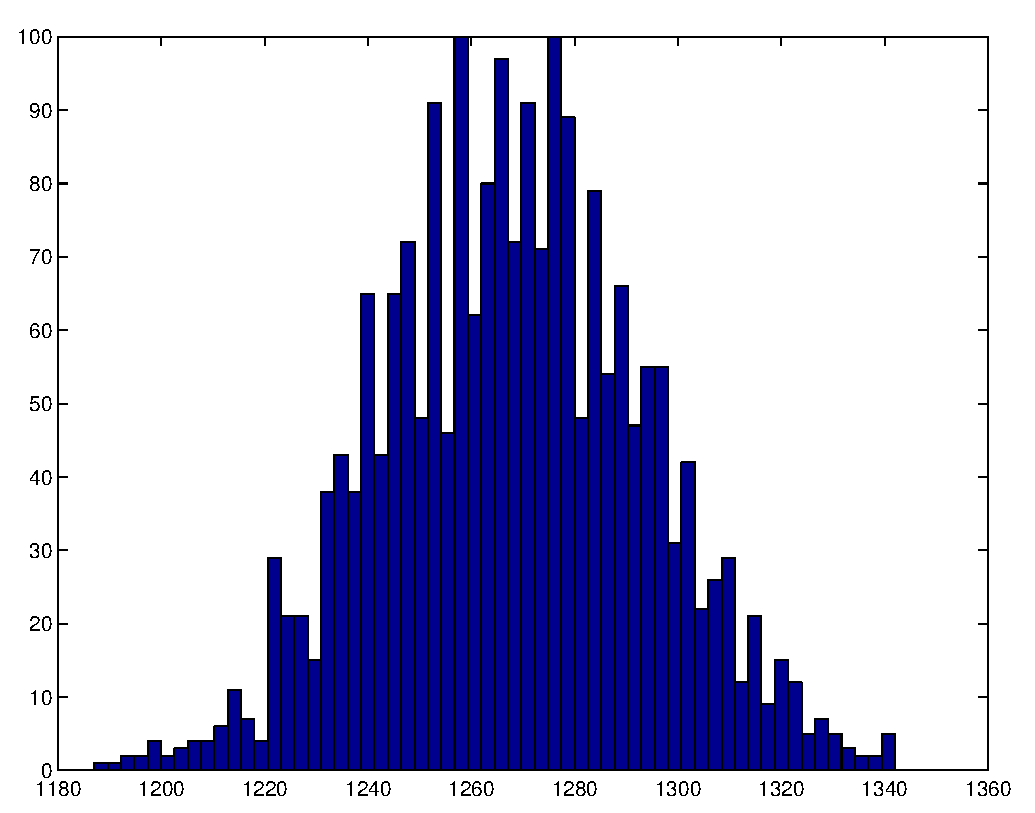
\includegraphics[width=\textwidth]{c_ic8_50Ks.eps}
%\caption{Distribution of final lengths given by the crowding simulation. See Table~\ref{tab:crowd} for details. 60 bin histogram for a sample of 2100.}
%\label{fig:crowd_ic8_50Ks}
%\end{figure}

\begin{figure}%[!htbp]
\centering
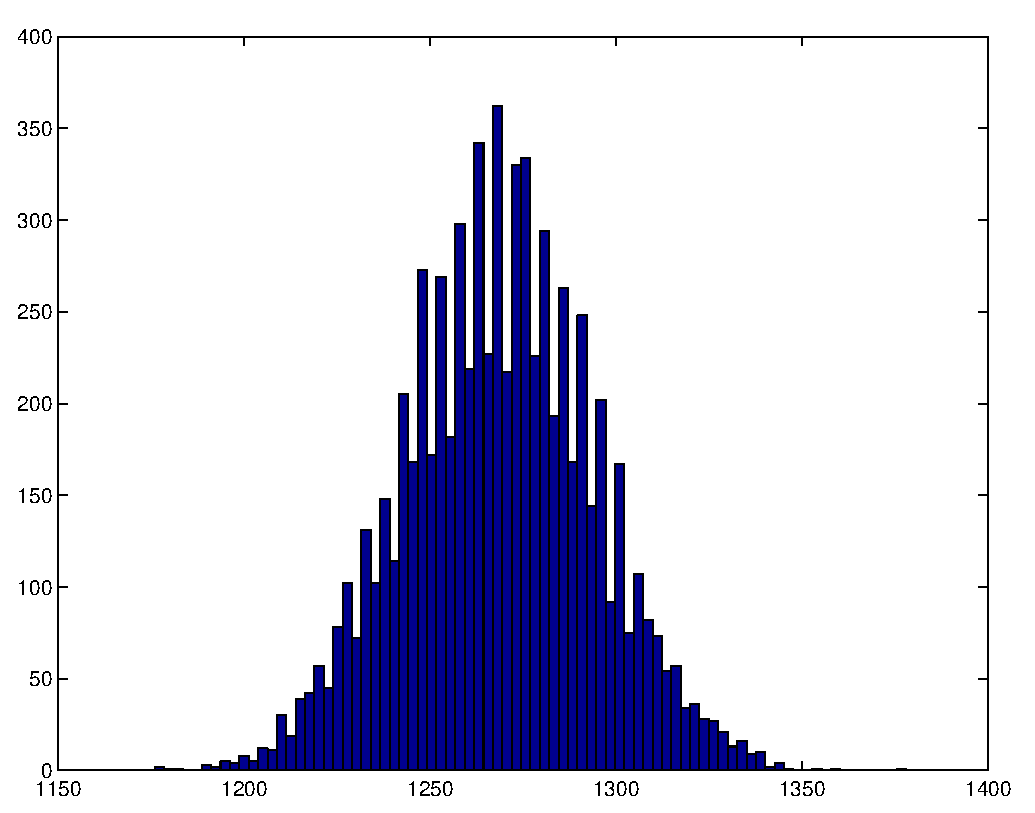
\includegraphics[height=3in]{c_ic8_15Ks}
\caption{Distribution of final lengths given by the crowding simulation.
The simulation was initialized at an initial length $N(0) = 1300$.
80 bin histogram for a sample size of 7280.}
\label{fig:crowd_ic8_15Ks}
\end{figure}

%\begin{figure}[!htbp]
%\centering
%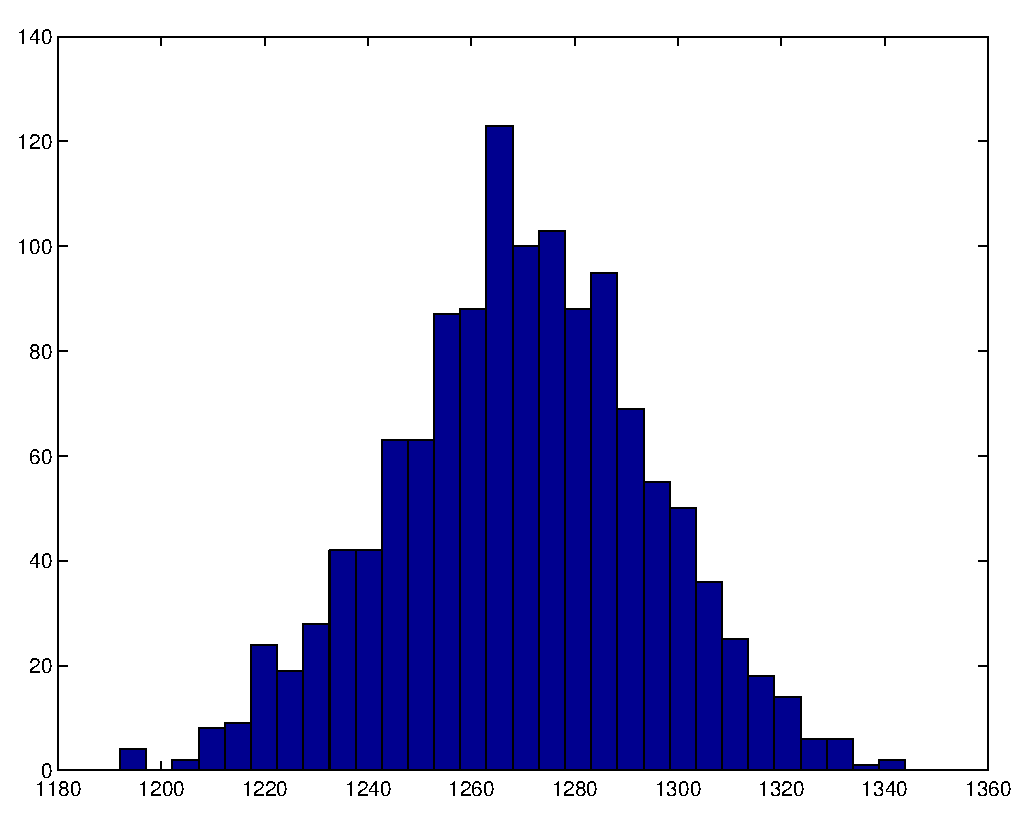
\includegraphics[width=\textwidth]{c_ic2_50Ks.eps}
%\caption{Distribution of final lengths given by the crowding simulation. See Table~\ref{tab:crowd} for details. 30 bin histogram for a sample of 1270.}
%\label{fig:crowd_ic2_50Ks}
%\end{figure}

%\begin{figure}[!htbp]
%\centering
%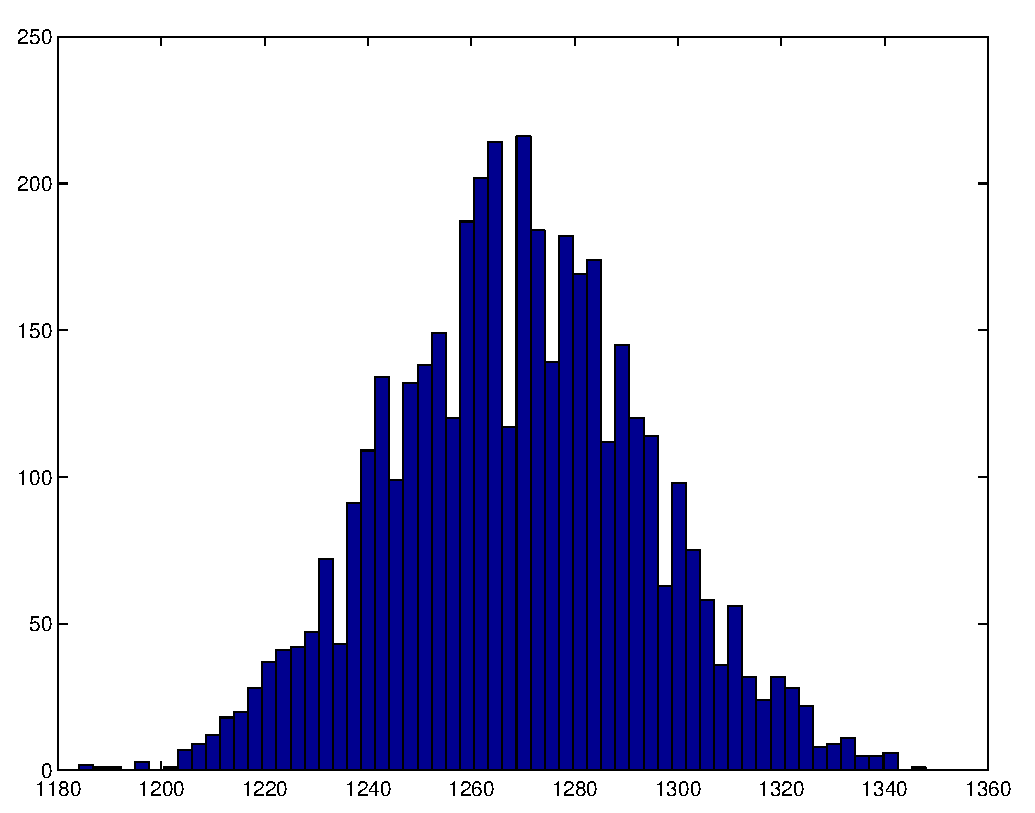
\includegraphics[width=\textwidth]{c_ic2_15Ks.eps}
%\caption{Distribution of final lengths given by the crowding simulation. See Table~\ref{tab:crowd} for details. 60 bin histogram for a sample of 4200.}
%\label{fig:crowd_ic2_15Ks}
%\end{figure}

\subsubsection{Comparing Different Distributions}
%The Kolmogorov-Smirnov test cannot reject the hypothesis that two samples come from the same distribution when any pair of samples from Table~\ref(tab:crowd).
According to the Kolmogorov-Smirnov test, the same final distribution are reached by trajectories run from different initial conditions.
Similarly, the test cannot reject the hypothesis that distributions at 15000s and at 50000s are the same.

\subsection{Crowding vs. Non-Crowding}
Since the crowding model yields a lower mean for the stationary distribution, it is clear that the two models do not give strictly the same distribution.
However, when the distributions are shifted so that their means match, the Kolmogorov-Smirnov test cannot reject the hypothesis that the two samples (one from the crowding model and one from the original model) come from the same distribution.

\section{Naive Birth-Death Model}

Due to the complexity of the discrete model, it is of interest whether this model can be simplified.
We are particularly interested in the length of the flagellum as a function of time, and the stationary distribution of the length, hence we attempt to write a model that is dependent on length and time alone.

One of the simpler forms of such a model is a birth-death model (see~\cite{ross} for a definition) where the death rate is the rate of disassembly and the birth rate is the total rate of assembly.

\subsection{Exact Stationary PDF Derivation}

In the birth-death model the state number $n$ represents the length of the flagellum in number of proteins ($N$ from the discrete model), the birth rate is the assembly rate, and the death rate is the disassembly rate.

The assembly rate is indicated in the ODE: since the frequency at which one transporter will arrive at the end of the flagellum with proteins for assembly is the mean speed of the transporter, $\bar{v}$, divided by the total distance to be traveled from the tip down and back to the tip again, $2 L$.
The frequency of assembly with $M$ transporters will then be $M$ times that rate, giving an assembly rate of $\frac{M \bar{v}}{2 L}$, or, using the notation in the discrete model, $\frac{M \bar\lambda}{2 N}$.
The disassembly rate is similarly simply $\mu$ from the discrete model.

From this we can get the following balance conditions for all positive-numbered states:

\begin{equation*}
 \mu \pi_{n+1} = \frac{M \bar\lambda }{2 n} \pi_n \qquad \forall n > 0
\end{equation*}

Since the rate of assembly is inversely proportional to the length (and the state number), there is a question of what the rate of assembly should be when the length is zero. For example, if we allow for the rate of assembly at zero to be the same as the rate of assembly at 1, we get a Poisson Distribution with mean equal to the ODE-predicted mean, since then we can get an expression for $\pi_n$ in terms of $\pi_0$:
\begin{equation*}
 \pi_n = \left(\frac{M\bar\lambda}{2 \mu}\right)^n \frac{1}{n!} \pi_0
\end{equation*}
which allows us to get:
\begin{align*}
 \sum_{n=0}^\infty \pi_n
 &= \sum_{n=0}^\infty \left(\frac{M\bar\lambda}{2 \mu}\right)^n \frac{1}{n!} \pi_0 \\
 &= \pi_0 e^{\frac{M\bar\lambda}{2 \mu}} \\
 &= 1
\end{align*}
giving:
\begin{equation*}
 \pi_n = e^{-(\frac{M\bar\lambda}{2 \mu})} \left(\frac{M\bar\lambda}{2 \mu }\right)^n \frac{1}{n!}
\end{equation*}
meaning that the stationary distribution is Poisson with mean and variance equal to the ODE mean.

Another possible value for the assembly rate at zero can be taken from the detailed simulation: When the length is zero all transporters are at the same position, all are moving anterograde, and once any transporter moves assembly will occur. Hence the rate of assembly will be the number of transporters $M$ times the anterograde movement rate, $\lambda_+$.

\begin{equation*}
 M \lambda_+ \pi_0 = \mu \pi_1
\end{equation*}

\begin{align*}
 \forall n > 0: \\
 \pi_{n+1} &= \frac{M \bar\lambda}{2 \mu n} \pi_n \\
 \pi_n &= \left( \frac{M \bar\lambda}{2 \mu} \right)^{n-1} \frac{1}{n!} \pi_1
\end{align*}

\begin{align*}
 \sum_{n = 0}^\infty \pi_n
 &= \pi_0 + \sum_{n = 1}^\infty \left( \frac{M \bar\lambda}{2 \mu} \right)^{n-1} \frac{1}{n!} \pi_1 \\
 &= \pi_0 + \sum_{n = 1}^\infty \left( \frac{M \bar\lambda}{2 \mu} \right)^{n} \frac{2 \mu}{M \bar\lambda} \frac{1}{n!} \pi_1 \\
 &= \pi_0 + \left( e^\frac{M \bar\lambda}{2 \mu} - 1 \right) \frac{2 \mu}{M \bar\lambda} \pi_1 \\
 &= \pi_0 \left( 1 + \left( e^\frac{M \bar\lambda}{2 \mu} - 1 \right) \frac{2 \mu}{M \bar\lambda} \frac{M \lambda_+}{\mu} \right) \\
 &= \pi_0 \left( 1 + \left( e^\frac{M \bar\lambda}{2 \mu} - 1 \right) \frac{2 \lambda_+}{\bar\lambda} \right) \\
 &= 1
\end{align*}

\begin{equation*}
\pi_0 = \frac{1}{ 1 + \left( e^\frac{M \bar\lambda}{2 \mu} - 1 \right) \frac{2 \lambda_+}{\bar\lambda} }
\end{equation*}

\begin{equation*}
\forall n > 0 \qquad \pi_n = \frac{M \lambda+}{ \left( 1 + \left( e^\frac{M \bar\lambda}{2 \mu} - 1 \right) \frac{2 \lambda_+}{\bar\lambda} \right) \mu n! } \left( \frac{M \bar\lambda}{2 \mu} \right)^{n-1}
\end{equation*}

Note that the resulting distribution is very similar to a Poisson distribution in shape.
In fact, the only difference is that the probability that $n=0$ is different, and the probabilities for $n>0$ are a constant multiple of the Poisson probabilities for $n>0$.
Additionally, noting that $\frac{M\bar\lambda}{2\mu} \gg 1$, and that $2\lambda_+ / \bar\lambda = 1 + ( \lambda_+ / \lambda_- ) > 1$, we can see that
\begin{equation*}
( 1 + ( e^\frac{M\bar\lambda}{2\mu} - 1 ) \frac{2 \lambda_+}{\bar\lambda} )
\approx \frac{2 \lambda_+}{\bar\lambda} e^\frac{M\bar\lambda}{2\mu}
\end{equation*}
Which means that the distribution is very close to a Poisson distribution, that is, the scaling is not very significant.

The birth-death model gives a stationary distribution with a variance of $\bar{N}$, which is about twice the variance observed from simulations of the detailed model.

\subsection{Simulation Results}
Figure~\ref{fig:bdTrajs} shows that the trajectory of the birth-death model does not match the ODE like the detailed stochastic model does; however, it does approach the same mean in the long run.
The major difference between the models is the fact that the standard deviation predicted by the birth-death model is twice the standard deviation observed from simulations of the detailed model.

\begin{figure}%[!htbp]
\centering
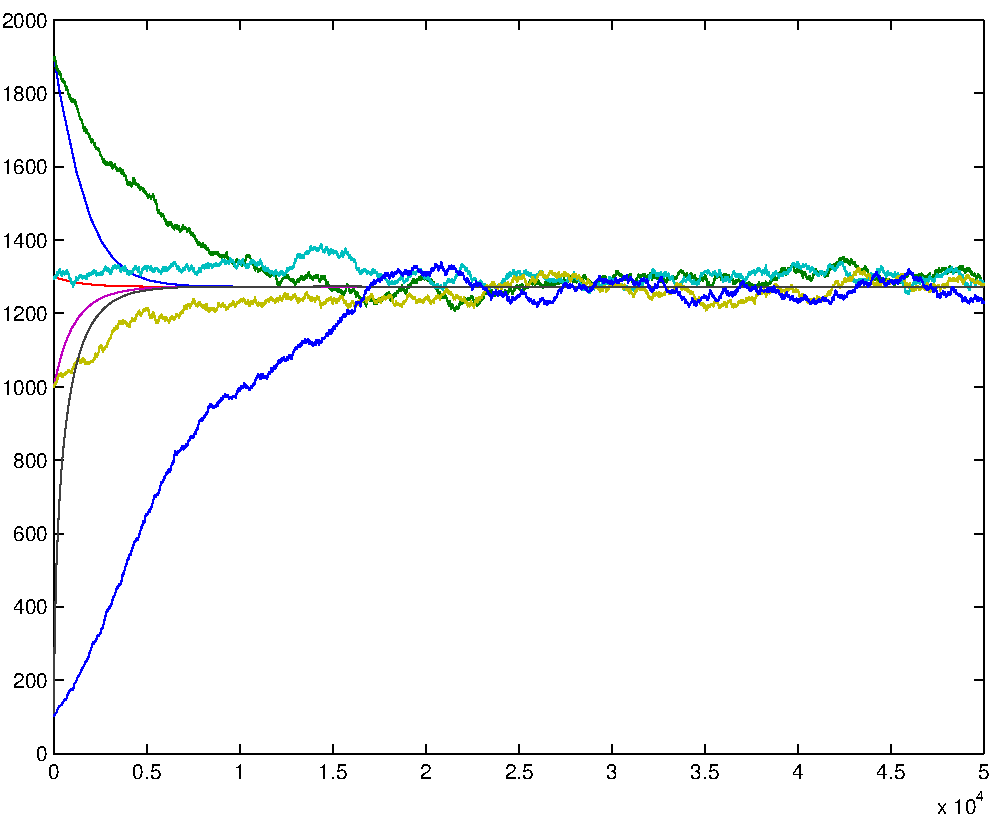
\includegraphics[width=\textwidth]{BirthDeathTrajs}
\caption{
Four representative trajectories generated by the birth-death simulation and corresponding solutions to the ODE.
The four different trajectories start from four different initial lengths: 100, 1000, 1300, and 1900, running to a time limit of 50000.
}
\label{fig:bdTrajs}
\end{figure}

\section{Stochastic Differential Equation Model}

After seeing that the simple birth-death model is inadequate, we try a different approach, which yields a stochastic differential equation (SDE) of the length as a function of time.

First, consider a time interval $[t,t+\tau]$, where $\tau$ is small enough so that the length of the flagellum $L$, and hence the number of segments $N$, does not change appreciably.
Denote the number of assemblies performed by transporter $i$ during the time interval $[t,t+\tau]$ by $X_i(\tau)$, $i=1,...,M$.

In a model without crowding effects, since the transporters are only affected by each other via the changing length of the flagellum, our assumption that $N$ does not change appreciably during the time interval allows us to say that $X_1(\tau),...,X_n(\tau)$ are almost i.i.d. random variables.

Treating $X_i(\tau)$ as a renewal process (see Ross~\cite{ross} for the definition of a renewal process) where $T_i$ is the random waiting time between increments of $X_i(\tau)$, we can find the mean and variance of the renewal time $T_i$ as follows:
To guarantee an assembly, the transporter must complete an entire loop around the flagellum, consisting of $N$ anterograde jumps and $N$ retrograde jumps. Using the notation from Section~\ref{sec:OriginalModel}, we can express $T_i$ as:

\begin{equation*}
T_i = \sum_{x=0}^N{T_{i,x+}} + \sum_{x=0}^N{T_{i,x-}}
\end{equation*}

Since the times between individual jumps $T_{i,x+}$ and $T_{i,x-}$ are independent exponential random variables with rates $\lambda_+$ and $\lambda_-$ respectively, the mean of one assembly can be expressed as the sum of their means:

\begin{equation*}
\E(T_i) = \sum_{x=0}^N{\E(T_{i,x+})} + \sum_{x=0}^N{\E(T_{i,x-})} = N \frac{1}{\lambda_+} + N \frac{1}{\lambda_-} = \frac{2N}{\bar{\lambda}}
\end{equation*}

And the variance can be expressed as:
\begin{equation*}
\var(T_i) = \sum_{x=0}^N{\var(T_{i,x+})} + \sum_{x=0}^N{\var(T_{i,x-})} = N \frac{1}{\lambda_+^2} + N \frac{1}{\lambda_-^2} = \frac{2N}{{\lambda^*}^2}
\end{equation*}

Where $\bar{\lambda}$ is the harmonic mean of $\lambda_+$ and $\lambda_-$, and $\lambda^*$ is defined as $\sqrt{\frac{2}{(\frac{1}{\lambda_+})^2+(\frac{1}{\lambda_-})^2}}$.

We now suppose that the time interval $[t,t+\tau]$ is such that the number of assemblies that the transporter performs in the time interval, $X_i(\tau)$, is sufficiently large to make use of the central limit theorem for renewal processes (see Appendix~\ref{sec:ren}).

We use the central limit theorem for renewal processes to approximate $X_i(\tau)$, as a normal distribution with mean and variance given by:

\begin{equation*}
\frac{\E(X_i(\tau))}{\tau}
\approx \lim_{s \to \infty}\frac{\E(X_i(s))}{s}
= \frac{1}{\E(T_i)}
= \frac{\bar{\lambda}}{2N}
\end{equation*}

\begin{equation*}
\frac{\var(X_i(\tau))}{\tau}
\approx \lim_{s \to \infty}\frac{\var(X_i(s))}{s}
= \frac{\var(T_i)}{\E^3(T_i)}
= \frac{2N}{{\lambda^*}^2} \left(\frac{\bar{\lambda}}{2N}\right)^3
= \frac{\bar{\lambda}^3}{4N^2{\lambda^*}^2}
\end{equation*}

Hence we can say that:
\begin{equation*}
X_i(\tau) \sim \Normal\left( \frac{\bar{\lambda}}{2N}\tau, \frac{\bar{\lambda}^3}{4N^2{\lambda^*}^2}\tau \right)
\end{equation*}

In the same interval of time $[t, t+\tau]$, the number of disassemblies, denoted by $Y(\tau)$ is Poisson with mean and variance $\mu\tau$.
When $\tau$ is large enough, this can also be approximated by a normal distribution with mean and variance $\mu\tau$.
Hence $Y(\tau) \sim \Normal(\mu\tau,\mu\tau)$.

We can then write an expression for the change in length during the time interval $[t,t+\tau]$:
\begin{equation*}
\delta N = N(t+\tau) - N(t) = \sum_{i=1}^M{X_i(\tau)} - Y(\tau)
\end{equation*}

Since $X_i(\tau)$ are almost i.i.d. and independent from $Y(\tau)$, $\delta N$ is a linear combination of mutually independent normal distributions and is therefore itself a normal distribution:
\begin{equation*}
\delta N \sim \Normal\left( \frac{M\bar{\lambda}\tau}{2N} - \mu\tau, \frac{M\bar{\lambda}^3\tau}{4N^2{\lambda^*}^2} + \mu\tau \right)
\end{equation*}
 
Which can be rewritten as an SDE for $N(t)$:

\begin{equation*}
dN(t) = \left( \frac{M\bar{\lambda}}{2N(t)} - \mu \right)dt + \sqrt{ \frac{M \bar{\lambda}^3}{4N^2(t){\lambda^*}^2} + \mu } \phantom{.} dB(t)
\end{equation*}

Where $B(t)$ is Brownian motion.

Recalling that we used a conversion from physical units of length to multiples of the segment length $a$, we can convert the SDE back to physical units of length ($dN(t) = dL(t)/a$, $(\bar{\lambda}) = (\bar{v})/a$, $\lambda^* = v^*/a$, $\mu = V/a$)

\begin{equation*}
dL(t) = \left( \frac{M\bar{v}a}{2L(t)} - V \right)dt + \sqrt{ \frac{M \bar{v}^3a^3}{4L^2(t){v^*}^2} + aV } \phantom{.} dB(t)
\end{equation*}

\subsection{SDE Simulation}

To compare the results predicted by the SDE to the results given by the (Non-Crowding) Monte Carlo simulation we use Euler's method to simulate the SDE trajectories.

Euler's method for solving an ODE such as $dy(x) = f(y(x))dx$ consists of viewing the ODE as a difference equation
\[ y(x_n) - y(x_{n-1}) = f(y(x_{n-1}))\cdot(x_n - x_{n-1}) \]
for some constant step size $(x_n - x_{n-1})$.
Similarly, we can view the SDE as a difference equation of random variables, that is, for the SDE
\[ dN(t) = f(N(t))dt + g(N(t))dB \]
we have a difference equation:
\[ N(t_n) - N(t_{n-1}) = f(N(t_{n-1}))\cdot(t_n - t_{n-1}) + g(N(t_{n-1}))\cdot(B(t_n) - B(t_{n-1})) \]
where $(B(t_n) - B(t_{n-1})) \sim \Normal(0, t_n - t_{n-1})$ by the properties of Brownian motion.
Then by choosing a step size $(t_n - t_{n-1})$ and an initial condition $N(0)$ we can simulate the SDE by generating random numbers for the Brownian motion term and iteratively generating $N(t_n)$ for each $n$.

\begin{figure}%[!htbp]
\centering
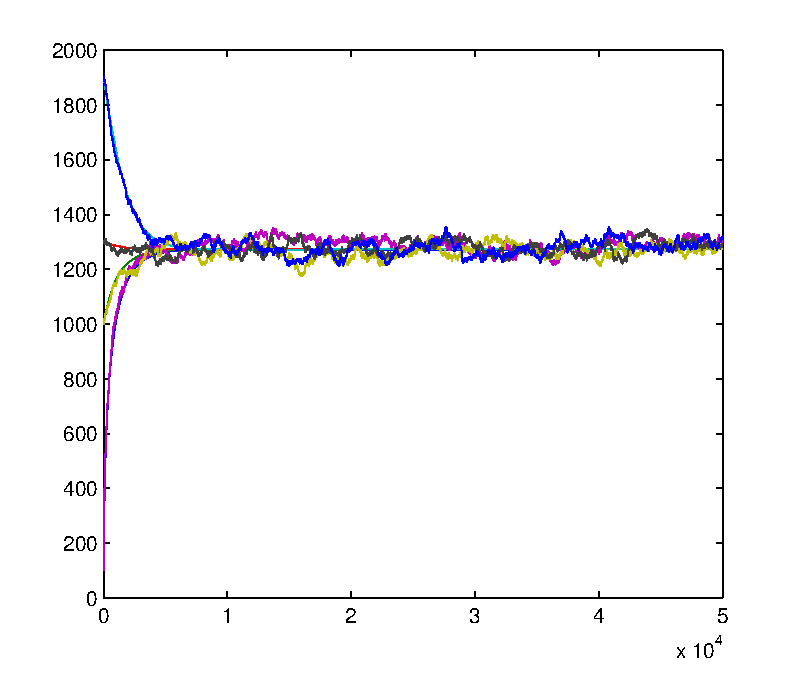
\includegraphics[width=\textwidth]{SDEtraj}
\caption{
Four representative SDE trajectories generated using Euler's method and corresponding solutions to the ODE.
The four different trajectories start from four different initial lengths: 100, 1000, 1300, and 1900, running to a time limit of 50000.}
\label{fig:SDEtraj}
\end{figure}

In the same manner in which we could generate a distribution for the length of the flagellum at a given time by running the Monte Carlo trajectories repeatedly and recording final length, we generate a distribution for the length of the flagellum at a given time by simulating a large number of trajectories for the SDE.

\begin{figure}%[!htbp]
\centering
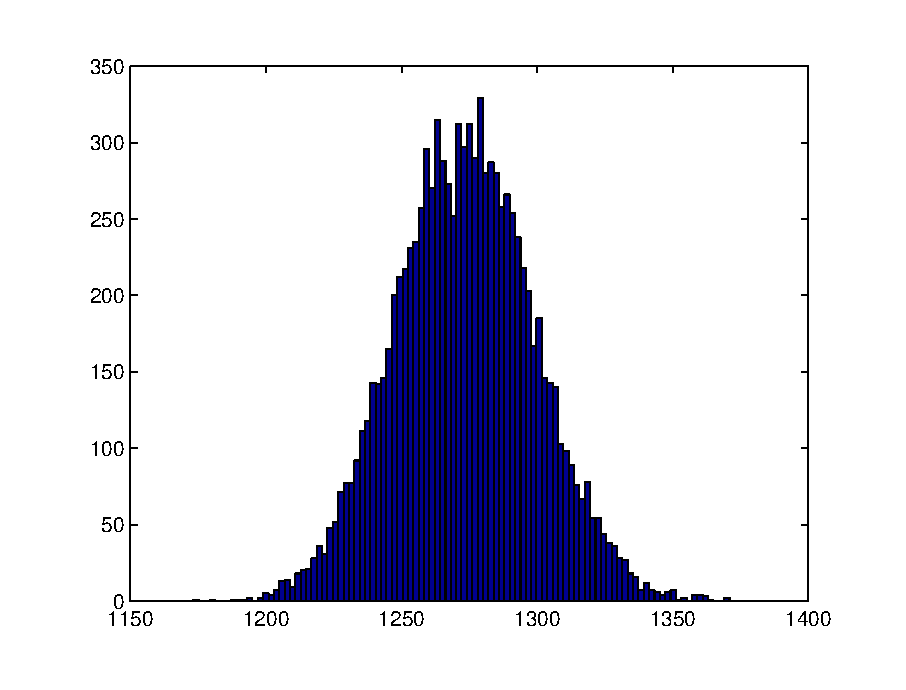
\includegraphics[height=3in]{SDEdist}
\caption{
Distribution of final lengths given by the SDE simulation.
The initial length was set to $N(0)=700$ and the time limit was set to 15000 seconds.
100 bin histogram for a sample size of 10000.
Mean: 1273.4
Standard deviation: 25.6482 }
\label{fig:SDEens}
\end{figure}

%Since the SDE suggests that the distribution is lognormal, and since the mean of the distribution is large, in finding how well the distributions agree, it is useful to approximate the distribution as normal, which allows us to compare confidence intervals for the mean and standard deviation of the distribution.
Since the distributions produced by the models and the distribution predicted by the SDE resemble Gaussians, we used the Gaussian assumption to compute the confidence intervals for the means and standard deviations of the simulation results.
The distribution generated by the SDE simulation has a mean and standard deviation that is within the confidence intervals corresponding to distributions from the detailed stochastic model (see Table~\ref{tab:ci}).

\section{Linear Noise Approximation}

Although the SDE simulation can be used to get the variance of the stationary distribution of flagellum lengths given a specific set of parameters, we are interested in getting an expression for the variance analytically.
For this purpose, we approximate the SDE with a linear noise approximation.

First we observe that near the equilibrium length, $\bar{N}$, the diffusion due to the assembly rate is very small.
Recall that $\bar{N}=\frac{\bar\lambda M}{2\mu}$.
Then:

\begin{align*}
\frac{M \bar{\lambda}^3}{4\bar{N}^2{\lambda^*}^2}
&= \frac{M \bar{\lambda}^3}{4{\lambda^*}^2}\left(\frac{2\mu}{\bar\lambda M}\right)^2 \\
&= \frac{\mu^2 \bar\lambda}{{\lambda^*}^2 M} \\
%\frac{M \bar{\lambda}^3}{4\bar{N}^2{\lambda^*}^2}
&\ll \mu
\end{align*}
since $\mu$ is orders of magnitude smaller than $\lambda_+$ and $\lambda_-$, and since $\frac{\bar\lambda}{\lambda^*}$ is bounded.

We can then rewrite the SDE near $N = \bar{N}$ as
\begin{equation*}
dN(t)=A(N(t))dt+\sqrt{\mu}dB(t)
\end{equation*}
where
\begin{equation*}
A(N(t)) := \left( \frac{M\bar{\lambda}}{2N(t)} - \mu \right)
\end{equation*}
Then let $\triangle N(t) := N(t)-\bar{N}$, which gives:
\begin{align*}
d \triangle N(t) = dN(t)
&= A(N(t))dt + \sqrt{\mu}dB(t) \\
&= A(\bar{N} + \triangle N(t))dt + \sqrt{\mu}dB(t)
\end{align*}
Taylor expanding $A(\bar{N} + \triangle N(t))$ around $\bar{N}$, and omitting terms after the second (since we are considering the case where $\triangle N(t)$ is small):
\begin{equation*}
d \triangle N(t) \approx
A(\bar{N}) + A'(\bar{N}) \triangle N(t)dt +  \sqrt{\mu}dB(t)
\end{equation*}
Observing that
\begin{align*}
A(\bar{N})
&= \frac{M\bar{\lambda}}{2\bar{N}} - \mu \\
&= \frac{M\bar{\lambda}}{2} \frac{2\mu}{\bar\lambda M} - \mu \\
&= \mu - \mu \\
A(\bar{N}) &= 0
\end{align*}
The above gives us the following linear SDE for the perturbation:
\begin{equation*}
d \triangle N(t) =
-\frac{M\bar\lambda}{2\bar{N}^2} \triangle N(t)dt + \sqrt{\mu}dB(t)
\end{equation*}

By taking the expectation of both sides, using linearity of expectation, and noting that $\E dB(t) = 0$ we get an ODE for $\E \triangle N(t)$:
\begin{equation*}
d \E \triangle N(t) =
-\frac{M\bar\lambda}{2\bar{N}^2} \E( \triangle N(t) )dt + \sqrt{\mu} \E( dB(t) )
\end{equation*}
\begin{equation*}
\frac{d \E( \triangle N(t) )}{dt} +
\frac{M\bar\lambda}{2\bar{N}^2} \E( \triangle N(t) )
= 0
\end{equation*}
Solving the equation gives:
\begin{equation*}
\E \triangle N(t) = C \exp \left( -\frac{M\bar\lambda}{2\bar{N}^2} t \right)
\end{equation*}
Taking the limit gives:
\begin{equation*}
\lim_{t \rightarrow \infty} \E \triangle N(t) = 0
\end{equation*}

Similarly, we can get an ODE and a solution for $\E( (\triangle N(t))^2 )$ (see Appendix~\ref{sec:deriv}).
This allows us to arrive at an expression for $\var( N(t) )$ as $t \rightarrow \infty$, and noting that $\E(N(t)) \rightarrow \bar{N}$:

\begin{align*}
\var( N(t) ) &= \E( ( N(t) - \E(N(t)) )^2 ) \\
&= \E( ( \bar{N} + \triangle N(t) - \bar{N} )^2 ) \\
&= \E( (\triangle N(t))^2 ) \\
\var( N(t) ) &\rightarrow \frac{M \bar{\lambda}}{4 \mu}
\qquad \textrm{as } t \rightarrow \infty
\end{align*}

Note that the above shows that the variance of the stationary distribution is approximated to be half the mean.
Table~\ref{tab:ci} compares different data from the discrete model and nonlinear SDE simulations to the mean and variance predicted by this approximation through the use of confidence intervals.
It can be seen that the distributions are close, and in most cases their means and variances are in each other's confidence intervals.

\begin{table}%[!htbp]
\centering
\begin{tabular}{c|rrr|cc}
 Model & \multicolumn{1}{c}{$N(0)$} & \multicolumn{1}{c}{Time Limit}
 & \multicolumn{1}{c}{Data} &
 \multicolumn{2}{c}{95\% Confidence Intervals for} \\
 & & \multicolumn{1}{c}{(seconds)} & \multicolumn{1}{c}{Points}
 & \multicolumn{1}{c}{Mean} &
 \multicolumn{1}{c}{Standard Deviation}
\\ \hline
 LNA & & & & 1272.7 & 25.2262 \\
 SDE & 100 & 15000 & 5000 & [1272.4, 1273.8] & [24.6917, 25.6790] \\
 SDE & 700 & 15000 & 100000 & [1273.1, 1273.4] & [25.1371, 25.3584]\\
 MAR & 100 & 15000 & 5000 & [1272.3, 1273.7] & [24.8236, 25.8162] \\
 MAR & 100 & 50000 & 3500 & [1271.1, 1272.7] & [24.5804, 25.7598] \\
 MAR & 1300 & 15000 & 5000 & [1271.6, 1273.0] & [24.7931, 25.7845] \\
 MAR & 1300 & 50000 & 2400 & [1272.1, 1274.1] & [24.4120, 25.8336]

\end{tabular}
\caption{Confidence intervals from various distributions.
The models are as follows:
LNA---linear noise approximation (only the mean and the variance, as calculated above, are given);
SDE---nonlinear SDE simulation;
MAR---Markov Chain simulation.}
\label{tab:ci}
\end{table}

\section{Conclusion}

We see the discrete model for flagellar length that was based on a Markov Chain can be approximated well by a nonlinear SDE that showed that the mean flagellum length predicted by the ODE a can be further approximated by a linear SDE.
The linear SDE was used to show that as long as the mean flagellar length is significantly greater than the length added by each transporter, and as long as the degeneration rate is much lower than the rates at which transporters move, the stationary distribution of the flagellum length has a variance of about half the mean.
This also provides an example of an instance where a simple birth-death model constructed from an ODE is inadequate (since the birth-death model yields a distribution with equal mean and variance).

It should be noted that although in the Markov Chain model we assumed the waiting times for transporters to move from one point to the next to be exponentially distributed random variables, since the SDE approximation makes use of the Central Limit Theorem for Renewal Processes, this approximation still holds for a more general case where those waiting times have variances equal to their mean squared.
The process of approximation here can also be generalized further for waiting times of any given mean and variance, yielding SDEs in terms of those means and variances.

Here we concentrated on the model's behavior near it's equilibrium.
It may be of interest to study how the model behaves at the other extreme, how fast it reaches its equilibrium, and what parameters affect these behaviors.
It would also be of interest to look for biological confirmation of the accuracy of this model (or the lack thereof).

\appendix

\section{Renewal Processes}\label{sec:ren}

\begin{clthm}[Ross~\cite{ross}, 7.3]
Let $\{N(t), t \leq 0 \}$ be a renewal process and let $\mu$ and $\sigma$ be, respectively, the mean and standard deviation of the interarrival distribution. Then the following holds:

\begin{equation*}
\lim_{t \rightarrow \infty} P \left\{
\frac{N(t)-t/\mu}{\sqrt{t\sigma^2/\mu^3}} < x
\right\}
= \frac{1}{\sqrt{2\pi}} \int_{-\infty}^x e^{-x^2/2} dx
\end{equation*}
\end{clthm}

Note that this means that as $t \rightarrow \infty$, $N(t)$ approaches a normal distribution with mean $\frac{1}{\mu}t$ and variance $\frac{\sigma^2}{\mu^3}t$, or, equivalently:
\begin{equation*}
\lim_{t \rightarrow \infty} \frac{\E(N(t))}{t} = \frac{1}{\mu}
\end{equation*}
and
\begin{equation*}
\lim_{t \rightarrow \infty} \frac{\var(N(t))}{t} = \frac{\sigma^2}{\mu^3}
\end{equation*}

\section{ $\E( (\triangle N(t))^2 )$ derivation }\label{sec:deriv}

Given the equation
\begin{equation*}
d \triangle N(t) =
-\frac{M\bar\lambda}{2\bar{N}^2} \triangle N(t)dt + \sqrt{\mu}dB(t)
\end{equation*}
First, a change of notation is convenient.
Let
\begin{align*}
B_t &= B(t) \\
\xi_t &= \triangle N(t) \\
\alpha &= -\frac{M\bar\lambda}{2\bar{N}^2} \\
\beta &= \sqrt{\mu}
\end{align*}
Giving
\begin{equation*}
d \xi_t = \alpha \xi_t dt + \beta dB_t
\end{equation*}

At this point we make use of the \Ito Formula, in particular, the 1-dimensional \Ito formula, in order to calculate $d(\xi_t^2)$:
\begin{itoform}[{\O}ksendal~\cite{oksendal}, Theorem 4.1.2]
For an \Ito process $\xi_t$ given by
\begin{equation*}
d \xi_t = u_t \xi_t dt + v_t dB_t
\end{equation*}
Let $g(t,x) \in C^2([0,\infty) \times \mathbb{R})$ (i.e. $g$ is twice continuously differentiable on $[0,\infty) \times \mathbb{R}$). Then
\begin{equation*}
\zeta_t = g(t,\xi_t)
\end{equation*}
is again an \Ito process, and
\begin{equation*}
d\zeta_t = \frac{\partial g}{\partial t}(t,\xi_t)dt + \frac{\partial g}{\partial x}(t, \xi_t)d\xi_t + \frac{1}{2}\frac{\partial^2 g}{\partial x^2}(t,\xi_t) \cdotp (d\xi_t)^2
\end{equation*}
where $(d\xi_t)^2 = (d\xi_t) \cdotp (d\xi_t)$ is computed according to the rules
\begin{equation*}
dt \cdotp dt = dt \cdotp dB_t = dB_t \cdotp dt = 0~, \quad dB_t \cdot dB_t = dt
\end{equation*}
\end{itoform}

We apply this formula to the particular case when $g(t,x) = x^2$, and we get:
\begin{align*}
d \zeta_t &= 0 dt + 2 \xi_t d \xi_t + \frac{1}{2} 2 (d \xi_t)^2 \\
&= 2 \xi_t (\alpha \xi_t dt + \beta dB_t) + (\alpha \xi_t dt + \beta dB_t)(\alpha \xi_t dt + \beta dB_t) \\
&= 2 \alpha \xi_t^2 dt + 2 \beta \xi dB_t + \alpha^2 \xi_t^2 (dt \cdotp dt) + \alpha \beta \xi_t (dt \cdotp dB_t + dB_t \cdotp dt) + \beta^2 (dB_t \cdot dB_t) \\
&= 2 \alpha \zeta_t dt + 2 \beta \xi_t dB_t + \beta^2 dt
\end{align*}
Taking the expected value of both sides gives
\begin{equation*}
d \E( \zeta_t ) = \E( d \zeta_t )
= 2 \alpha \E( \zeta_t )dt + \beta^2 dt
\end{equation*}
The general solution to the resulting ODE is
\begin{equation*}
\E \zeta_t = C e^{-2\alpha t} - \frac{\beta^2}{2\alpha}
\end{equation*}
Then we can finally arrive at an expression for $\lim_{t \rightarrow \infty} \E( (\triangle N(t))^2 )$:
\begin{align*}
\lim_{t \rightarrow \infty} \E( (\triangle N(t))^2 )
&= \lim_{t \rightarrow \infty} \E \zeta_t \\
&= - \frac{\beta^2}{2\alpha} \\
&= \frac{\mu}{2}\frac{2\bar{N}^2}{M\bar\lambda} \\
&= \frac{\mu}{M\bar\lambda} \bar{N}^2 \\
&= \frac{\mu}{M\bar\lambda} \left( \frac{\bar\lambda M}{2\mu} \right)^2 \\
&= \frac{M\bar\lambda}{4\mu}
\end{align*}

\begin{thebibliography}{99}
\raggedright

\bibitem{bressloff}
Bressloff, P. C. (2006).
Stochastic model of intraflagellar transport.
\emph{Physical Review E, 73,} 061916.

\bibitem{matsumoto}
Matsumoto, M. (2007).
\emph{SIMD-oriented Fast Mersenne Twister (SFMT)}
Retrieved January 13, 2008, from 
\emph{Hiroshima University, Department of Mathematics} Web site, 
http://www.math.sci.hiroshima-u.ac.jp/$\sim$m-mat/MT/SFMT/index.html

\bibitem{oksendal}
{\O}ksendal, Bernt (2007).
\emph{Stochastic Differential Equations: And Introduction with Applications}
(6th ed.).
New York Berlin Heidelberg: Springer.

\bibitem{rosenbaum2}
Rosenbaum, Joel L. and Witman, George B. (2002).
Intraflagellar Transport.
\emph{Nature Reviews: Molecular Cell Biology, 3(11)}, 813-825.

\bibitem{rosenbaum}
\emph{Rosenbaum Lab Research Summary} (n. d.).
Retrieved January 25, 2008, from
\emph{Yale University, Deptartment of Molecular, Cellular, and Developmental Biology} Web site,  \mbox{
http://www.yale.edu/rosenbaum/rosen\_research.html}

\bibitem{ross}
Ross, S. M. (2007).
\emph{Introduction to probability models} (9th ed.).
San Diego, CA: Academic Press.

\end{thebibliography}


\end{document}
